\documentclass{article}
\usepackage{etex}

\usepackage{bytefield}
\usepackage{booktabs}
\usepackage{fancyhdr}
\usepackage{float}
\usepackage{graphicx}
\usepackage{helvet}
\usepackage{hyperref}
\usepackage{tabularx}
\usepackage{xcolor}
\usepackage{color, colortbl}

\usepackage{listings}
\usepackage{tikz}

\usepackage{makeidx}         % allows index generation
\makeindex

\lstset{frame=tblr,
  rulecolor=\color{lightgray},
  language=Java,
  aboveskip=5mm,
  belowskip=5mm,
  showstringspaces=false,
  columns=flexible,
  basicstyle=\linespread{1.0}\small\ttfamily,
  numbers=none,
  % numberstyle=\tiny\color{gray},
  % keywordstyle=\color{blue},
  % commentstyle=\color{dkgreen},
  % stringstyle=\color{mauve},
  breaklines=true,
  breakatwhitespace=true,
  tabsize=3
}

\usepackage{framed}     % These needed for the code formatter
\usepackage{color}
\usepackage{fancyvrb}

% Use helvetica (sans) by default
\renewcommand{\familydefault}{\sfdefault}

% Greenish links
\hypersetup{
  colorlinks=true,
  linkcolor=blue!50!red,
  urlcolor=blue!50!red
}

\newcommand{\two}{\raise0.5ex\hbox{\footnotesize{2}}}

\newcommand{\iic}{I\two{}C}
\newcommand{\iicdriver}{I\two{}CDriver}
\newcommand{\iicmini}{I\two{}CMini}
\newcommand{\degc}{$^{\circ}$C}
\newcommand{\device}{\iicdriver{}}

\setlength{\headheight}{40pt}
\setlength{\headsep}{0.2in}

\pagestyle{fancy}
\lhead{
\includegraphics[width=0.2\textwidth]{img/logo}}
\chead{\iicdriver{} and \iicmini{} User Guide}
\rhead{\thepage}
\cfoot{\textcopyright \the\year \ \ Excamera Labs}
\renewcommand{\headrulewidth}{0.5pt}
\renewcommand{\footrulewidth}{0.5pt}

\usepackage{array}
\newcolumntype{L}[1]{>{\raggedright\let\newline\\\arraybackslash\hspace{0pt}}m{#1}}
\newcolumntype{C}[1]{>{\centering\let\newline\\\arraybackslash\hspace{0pt}}m{#1}}
\newcolumntype{R}[1]{>{\raggedleft\let\newline\\\arraybackslash\hspace{0pt}}m{#1}}

\usepackage{setspace}

\newcommand{\heavyline}{\specialrule{1pt}{1pt}{1pt}}
\newcommand{\png}[1]{
\begin{figure}[H]
\begin{center}
\includegraphics[width=0.75\textwidth]{#1}
\end{center}
\end{figure}
}
\newcommand{\pngw}[2]{
\begin{figure}[H]
\begin{center}
\includegraphics[width=#2\textwidth]{#1}
\end{center}
\end{figure}
}

\usepackage{sphinx}

\newcommand{\mach}[1]{\texttt{\textbf{#1}}}
\newcommand{\gap}{\vspace{10pt}}

\newcommand\encircle[1]{%
  \tikz[baseline=(X.base)] 
   \node (X) [draw, shape=circle, inner sep=0] {\strut #1};}


\makeatletter
\def\PY@reset{\let\PY@it=\relax \let\PY@bf=\relax%
    \let\PY@ul=\relax \let\PY@tc=\relax%
    \let\PY@bc=\relax \let\PY@ff=\relax}
\def\PY@tok#1{\csname PY@tok@#1\endcsname}
\def\PY@toks#1+{\ifx\relax#1\empty\else%
    \PY@tok{#1}\expandafter\PY@toks\fi}
\def\PY@do#1{\PY@bc{\PY@tc{\PY@ul{%
    \PY@it{\PY@bf{\PY@ff{#1}}}}}}}
\def\PY#1#2{\PY@reset\PY@toks#1+\relax+\PY@do{#2}}

\expandafter\def\csname PY@tok@gd\endcsname{\def\PY@tc##1{\textcolor[rgb]{0.63,0.00,0.00}{##1}}}
\expandafter\def\csname PY@tok@gu\endcsname{\let\PY@bf=\textbf\def\PY@tc##1{\textcolor[rgb]{0.50,0.00,0.50}{##1}}}
\expandafter\def\csname PY@tok@gt\endcsname{\def\PY@tc##1{\textcolor[rgb]{0.00,0.27,0.87}{##1}}}
\expandafter\def\csname PY@tok@gs\endcsname{\let\PY@bf=\textbf}
\expandafter\def\csname PY@tok@gr\endcsname{\def\PY@tc##1{\textcolor[rgb]{1.00,0.00,0.00}{##1}}}
\expandafter\def\csname PY@tok@cm\endcsname{\let\PY@it=\textit\def\PY@tc##1{\textcolor[rgb]{0.25,0.50,0.50}{##1}}}
\expandafter\def\csname PY@tok@vg\endcsname{\def\PY@tc##1{\textcolor[rgb]{0.10,0.09,0.49}{##1}}}
\expandafter\def\csname PY@tok@m\endcsname{\def\PY@tc##1{\textcolor[rgb]{0.40,0.40,0.40}{##1}}}
\expandafter\def\csname PY@tok@mh\endcsname{\def\PY@tc##1{\textcolor[rgb]{0.40,0.40,0.40}{##1}}}
\expandafter\def\csname PY@tok@go\endcsname{\def\PY@tc##1{\textcolor[rgb]{0.53,0.53,0.53}{##1}}}
\expandafter\def\csname PY@tok@ge\endcsname{\let\PY@it=\textit}
\expandafter\def\csname PY@tok@vc\endcsname{\def\PY@tc##1{\textcolor[rgb]{0.10,0.09,0.49}{##1}}}
\expandafter\def\csname PY@tok@il\endcsname{\def\PY@tc##1{\textcolor[rgb]{0.40,0.40,0.40}{##1}}}
\expandafter\def\csname PY@tok@cs\endcsname{\let\PY@it=\textit\def\PY@tc##1{\textcolor[rgb]{0.25,0.50,0.50}{##1}}}
\expandafter\def\csname PY@tok@cp\endcsname{\def\PY@tc##1{\textcolor[rgb]{0.74,0.48,0.00}{##1}}}
\expandafter\def\csname PY@tok@gi\endcsname{\def\PY@tc##1{\textcolor[rgb]{0.00,0.63,0.00}{##1}}}
\expandafter\def\csname PY@tok@gh\endcsname{\let\PY@bf=\textbf\def\PY@tc##1{\textcolor[rgb]{0.00,0.00,0.50}{##1}}}
\expandafter\def\csname PY@tok@ni\endcsname{\let\PY@bf=\textbf\def\PY@tc##1{\textcolor[rgb]{0.60,0.60,0.60}{##1}}}
\expandafter\def\csname PY@tok@nl\endcsname{\def\PY@tc##1{\textcolor[rgb]{0.63,0.63,0.00}{##1}}}
\expandafter\def\csname PY@tok@nn\endcsname{\let\PY@bf=\textbf\def\PY@tc##1{\textcolor[rgb]{0.00,0.00,1.00}{##1}}}
\expandafter\def\csname PY@tok@no\endcsname{\def\PY@tc##1{\textcolor[rgb]{0.53,0.00,0.00}{##1}}}
\expandafter\def\csname PY@tok@na\endcsname{\def\PY@tc##1{\textcolor[rgb]{0.49,0.56,0.16}{##1}}}
\expandafter\def\csname PY@tok@nb\endcsname{\def\PY@tc##1{\textcolor[rgb]{0.00,0.50,0.00}{##1}}}
\expandafter\def\csname PY@tok@nc\endcsname{\let\PY@bf=\textbf\def\PY@tc##1{\textcolor[rgb]{0.00,0.00,1.00}{##1}}}
\expandafter\def\csname PY@tok@nd\endcsname{\def\PY@tc##1{\textcolor[rgb]{0.67,0.13,1.00}{##1}}}
\expandafter\def\csname PY@tok@ne\endcsname{\let\PY@bf=\textbf\def\PY@tc##1{\textcolor[rgb]{0.82,0.25,0.23}{##1}}}
\expandafter\def\csname PY@tok@nf\endcsname{\def\PY@tc##1{\textcolor[rgb]{0.00,0.00,1.00}{##1}}}
\expandafter\def\csname PY@tok@si\endcsname{\let\PY@bf=\textbf\def\PY@tc##1{\textcolor[rgb]{0.73,0.40,0.53}{##1}}}
\expandafter\def\csname PY@tok@s2\endcsname{\def\PY@tc##1{\textcolor[rgb]{0.73,0.13,0.13}{##1}}}
\expandafter\def\csname PY@tok@vi\endcsname{\def\PY@tc##1{\textcolor[rgb]{0.10,0.09,0.49}{##1}}}
\expandafter\def\csname PY@tok@nt\endcsname{\let\PY@bf=\textbf\def\PY@tc##1{\textcolor[rgb]{0.00,0.50,0.00}{##1}}}
\expandafter\def\csname PY@tok@nv\endcsname{\def\PY@tc##1{\textcolor[rgb]{0.10,0.09,0.49}{##1}}}
\expandafter\def\csname PY@tok@s1\endcsname{\def\PY@tc##1{\textcolor[rgb]{0.73,0.13,0.13}{##1}}}
\expandafter\def\csname PY@tok@sh\endcsname{\def\PY@tc##1{\textcolor[rgb]{0.73,0.13,0.13}{##1}}}
\expandafter\def\csname PY@tok@sc\endcsname{\def\PY@tc##1{\textcolor[rgb]{0.73,0.13,0.13}{##1}}}
\expandafter\def\csname PY@tok@sx\endcsname{\def\PY@tc##1{\textcolor[rgb]{0.00,0.50,0.00}{##1}}}
\expandafter\def\csname PY@tok@bp\endcsname{\def\PY@tc##1{\textcolor[rgb]{0.00,0.50,0.00}{##1}}}
\expandafter\def\csname PY@tok@c1\endcsname{\let\PY@it=\textit\def\PY@tc##1{\textcolor[rgb]{0.25,0.50,0.50}{##1}}}
\expandafter\def\csname PY@tok@kc\endcsname{\let\PY@bf=\textbf\def\PY@tc##1{\textcolor[rgb]{0.00,0.50,0.00}{##1}}}
\expandafter\def\csname PY@tok@c\endcsname{\let\PY@it=\textit\def\PY@tc##1{\textcolor[rgb]{0.25,0.50,0.50}{##1}}}
\expandafter\def\csname PY@tok@mf\endcsname{\def\PY@tc##1{\textcolor[rgb]{0.40,0.40,0.40}{##1}}}
\expandafter\def\csname PY@tok@err\endcsname{\def\PY@bc##1{\setlength{\fboxsep}{0pt}\fcolorbox[rgb]{1.00,0.00,0.00}{1,1,1}{\strut ##1}}}
\expandafter\def\csname PY@tok@kd\endcsname{\let\PY@bf=\textbf\def\PY@tc##1{\textcolor[rgb]{0.00,0.50,0.00}{##1}}}
\expandafter\def\csname PY@tok@ss\endcsname{\def\PY@tc##1{\textcolor[rgb]{0.10,0.09,0.49}{##1}}}
\expandafter\def\csname PY@tok@sr\endcsname{\def\PY@tc##1{\textcolor[rgb]{0.73,0.40,0.53}{##1}}}
\expandafter\def\csname PY@tok@mo\endcsname{\def\PY@tc##1{\textcolor[rgb]{0.40,0.40,0.40}{##1}}}
\expandafter\def\csname PY@tok@kn\endcsname{\let\PY@bf=\textbf\def\PY@tc##1{\textcolor[rgb]{0.00,0.50,0.00}{##1}}}
\expandafter\def\csname PY@tok@mi\endcsname{\def\PY@tc##1{\textcolor[rgb]{0.40,0.40,0.40}{##1}}}
\expandafter\def\csname PY@tok@gp\endcsname{\let\PY@bf=\textbf\def\PY@tc##1{\textcolor[rgb]{0.00,0.00,0.50}{##1}}}
\expandafter\def\csname PY@tok@o\endcsname{\def\PY@tc##1{\textcolor[rgb]{0.40,0.40,0.40}{##1}}}
\expandafter\def\csname PY@tok@kr\endcsname{\let\PY@bf=\textbf\def\PY@tc##1{\textcolor[rgb]{0.00,0.50,0.00}{##1}}}
\expandafter\def\csname PY@tok@s\endcsname{\def\PY@tc##1{\textcolor[rgb]{0.73,0.13,0.13}{##1}}}
\expandafter\def\csname PY@tok@kp\endcsname{\def\PY@tc##1{\textcolor[rgb]{0.00,0.50,0.00}{##1}}}
\expandafter\def\csname PY@tok@w\endcsname{\def\PY@tc##1{\textcolor[rgb]{0.73,0.73,0.73}{##1}}}
\expandafter\def\csname PY@tok@kt\endcsname{\def\PY@tc##1{\textcolor[rgb]{0.69,0.00,0.25}{##1}}}
\expandafter\def\csname PY@tok@ow\endcsname{\let\PY@bf=\textbf\def\PY@tc##1{\textcolor[rgb]{0.67,0.13,1.00}{##1}}}
\expandafter\def\csname PY@tok@sb\endcsname{\def\PY@tc##1{\textcolor[rgb]{0.73,0.13,0.13}{##1}}}
\expandafter\def\csname PY@tok@k\endcsname{\let\PY@bf=\textbf\def\PY@tc##1{\textcolor[rgb]{0.00,0.50,0.00}{##1}}}
\expandafter\def\csname PY@tok@se\endcsname{\let\PY@bf=\textbf\def\PY@tc##1{\textcolor[rgb]{0.73,0.40,0.13}{##1}}}
\expandafter\def\csname PY@tok@sd\endcsname{\let\PY@it=\textit\def\PY@tc##1{\textcolor[rgb]{0.73,0.13,0.13}{##1}}}

\def\PYZbs{\char`\\}
\def\PYZus{\char`\_}
\def\PYZob{\char`\{}
\def\PYZcb{\char`\}}
\def\PYZca{\char`\^}
\def\PYZam{\char`\&}
\def\PYZlt{\char`\<}
\def\PYZgt{\char`\>}
\def\PYZsh{\char`\#}
\def\PYZpc{\char`\%}
\def\PYZdl{\char`\$}
\def\PYZhy{\char`\-}
\def\PYZsq{\char`\'}
\def\PYZdq{\char`\"}
\def\PYZti{\char`\~}
% for compatibility with earlier versions
\def\PYZat{@}
\def\PYZlb{[}
\def\PYZrb{]}
\makeatother



\begin{document}

\newpage
\begin{center}
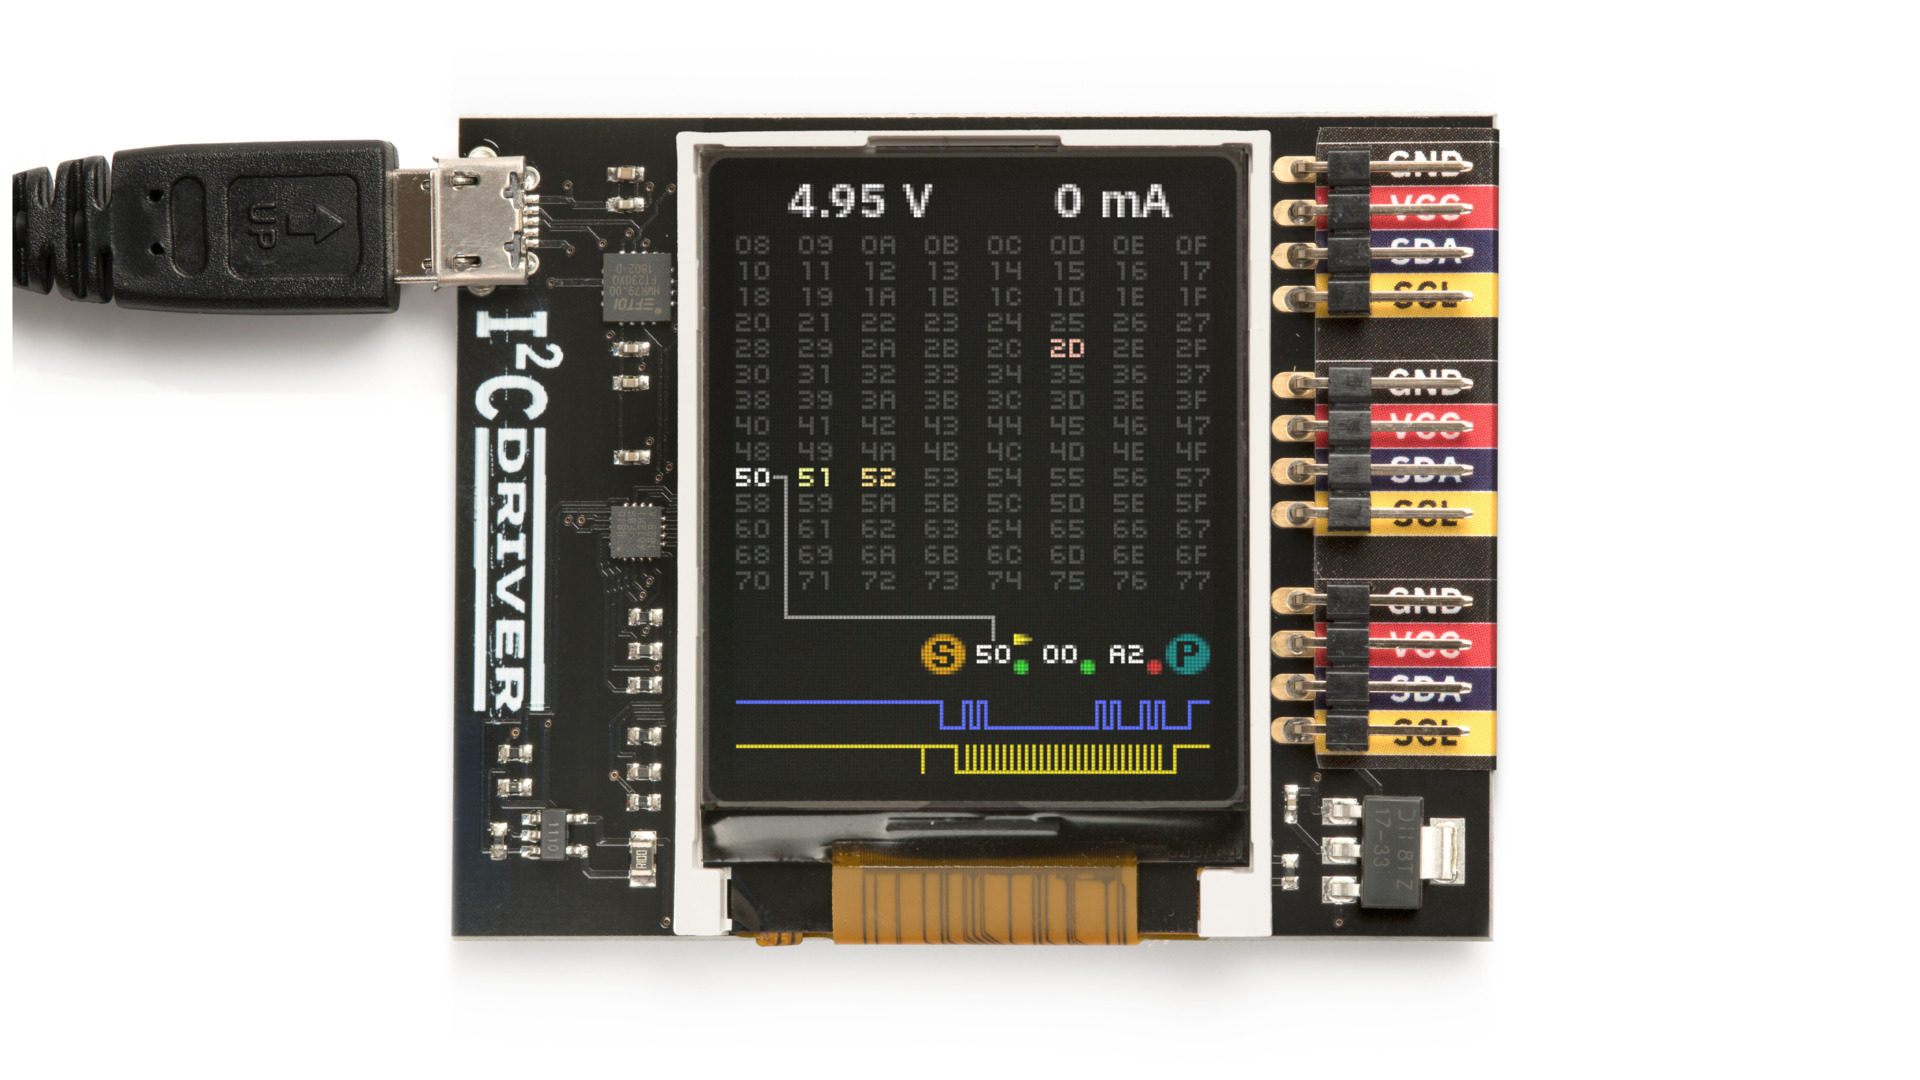
\includegraphics[width=1.00\textwidth]{img/i2cdriver/i2cdriver-hero}
Last updated on \today
\end{center}
\tableofcontents

\newpage

\setlength{\parindent}{0mm}
\setlength{\parskip}{1mm}
\setstretch{1.4}

\section{Overview}

\iicdriver{} is an easy-to-use, open source tool for controlling \iic{} devices.
It works with Windows, Mac, and Linux, and has a built-in color screen that shows a live “dashboard” of all the \iic{} activity.
It uses a standard FTDI USB serial chip to talk to the PC, so no special drivers need to be installed.
The board includes a separate 3.3 V supply with voltage and current monitoring.

\iicmini{} is a reduced-size version of \iicdriver{} suitable for use in embedded devices.
It is 100\% compatible with \iicdriver{} but lacks a display, current or voltage monitoring.
In every other respect it behaves identically to \iicdriver{}.

\subsection{Features}
\begin{itemize}
\item \textbf{Live display}: shows you exactly what it's doing all the time  
\item \textbf{Supports all \iic{} features}: 7- and 10-bit \iic{} addressing, clock stretching, bus arbitration,
and sustained \iic{} transfers at 400 and 100 kHz  
\item \textbf{\iic{} pullups}: programmable \iic{} pullup resistors, with automatic tuning  
\item \textbf{USB voltage monitoring}: USB line voltage monitor to detect supply problems, to 0.01 V  
\item \textbf{Target power monitoring}: target device high-side current measurement, to 5 mA  
\item \textbf{Three \iic{} ports}: three identical \iic{} ports, each with power and \iic{} signals  
\item \textbf{Jumpers}: three sets of high-quality color coded 100mm jumpers included
\item \textbf{3.3 V output}: output levels are 3.3 V, all are 5 V tolerant  
\item \textbf{Sturdy componentry}: uses an FTDI USB serial adapter, and Silicon Labs automotive-grade EFM8 controller  
\item \textbf{Open hardware}: the design, firmware and all tools are under BSD license
\item \textbf{Flexible control}: GUI, command-line, C/C++, and Python 2/3 host software provided for Windows, Mac, and Linux  
\end{itemize}

\newpage
\section{Getting Started}

When you first connect \iicdriver{} to the USB port, the display blinks white for a moment
then displays the initial status screen:

\png{img/i2cdriver/i2c_driver_cabled}

Connect the three sets of colored hookup wires as shown, \index{hookup}\index{jumpers}
following the same sequence as on the colored label:

\definecolor{ccGND}{gray}{0.0}
\definecolor{ccVCC}{RGB}{191, 13, 45}
\definecolor{ccSDA}{RGB}{  0, 32, 91}
\definecolor{ccSCL}{RGB}{255,215,  0}
\definecolor{white}{RGB}{255,255,255}

\gap
\begin{center}
\begin{tabular}{ccl}
\hline
\cellcolor{ccGND}
\textcolor{white}{\textbf{GND}}  & black & signal ground \\
\cellcolor{ccVCC}
\textcolor{white}{\textbf{VCC}}  & red & 3.3 V supply \\
\cellcolor{ccSDA}
\textcolor{white}{\textbf{SDA}}  & blue & \iic{} data \\
\cellcolor{ccSCL}
\textbf{SCL}  & yellow & \iic{} clock \\
\hline
\end{tabular}
\end{center}
\gap

Across the top of the display \iicdriver{} continuously shows
the USB bus voltage and the current output.

\png{img/i2cdriver/i2c_mini_topdown_wired_white_bg}

\iicmini{} also has a micro USB connector.
Its Qwiic connector is polarized; it attaches as shown.
\index{Qwiic}
The color coding for the signals is the same as for \iicdriver{}.

\newpage
\section{Software installation}

The source for all the \iicdriver{} software is the
\href{https://github.com/jamesbowman/i2cdriver}{repository}.
Available are:

\begin{itemize}
\item a Windows/Mac/Linux GUI
\item a Windows/Mac/Linux command-line
\item Python 2 and 3 bindings
\item Windows/Mac/Linux C/C++ bindings
\end{itemize}

Installation of the GUI and command-line utilities varies by platform.

\subsection{Windows}\index{drivers!Windows}

This
\href{https://i2cdriver.com/windows}{installer}
contains the GUI and command-line utilities.

The GUI shortcut is installed on the desktop:

\pngw{img/i2cdriver/win32-icon}{.3}

launching it brings up the control window:

\pngw{img/i2cdriver/win32-gui}{1.0}

If there is only one serial device, 
the \iicdriver{} device should be automatically selected.
If there is more than one device, select its COM port from the pulldown menu at the top.
Once connected, you can select a connected \iic{} device and write and read data. 

The command line utility \mach{i2ccl} is also installed,
and added to the Windows \mach{PATH}.
For example to display status information:

\begin{lstlisting}
c:\>i2ccl COM6 i
uptime 8991  4.957 V  30 mA  25.8 C SDA=1 SCL=1 speed=100 kHz
\end{lstlisting}

The COM port can be found using the \mach{MODE} command to list connected ports. \index{COM port}
You can use the Device Manager or the \mach{MODE} command to display the available ports.

The Windows convention for \mach{COM10} and above is that they must be prefixed by
\mach{\textbackslash\textbackslash.\textbackslash},
for example: \index{COM10 etc.} 

\begin{lstlisting}
c:\>i2ccl \\.\COM11 i
\end{lstlisting}

See (section \ref{portnames} "\nameref{portnames}") for details on how to fix a device to a port number permanently.

See below for more information on the command-line syntax.

\subsection{Linux}\index{drivers!Linux}

The GUI is included in the \mach{i2cdriver} Python package, compatible with both Python 2 and 3.
To install it, open a shell prompt and do:

\begin{lstlisting}
sudo pip install i2cdriver
\end{lstlisting}

Then run it with

\begin{lstlisting}
i2cgui.py
\end{lstlisting}

For the command-line tool, clone the
\href{https://github.com/jamesbowman/i2cdriver}{repository},
then do:

\begin{lstlisting}
cd i2cdriver/c
make -f linux/Makefile
sudo make -f linux/Makefile install
i2ccl /dev/ttyUSB0 i
\end{lstlisting}

and you should see something like:

\begin{lstlisting}
uptime 1651  4.971 V  0 mA  21.2 C SDA=1 SCL=1 speed=100 kHz
\end{lstlisting}

\subsection{MacOS}\index{drivers!Mac}

The GUI is included in the \mach{i2cdriver} Python package, compatible with both Python 2 and 3.
To install it, open a shell prompt and do:

\begin{lstlisting}
sudo pip install i2cdriver
\end{lstlisting}

Then run it with

\begin{lstlisting}
i2cgui.py
\end{lstlisting}

For the command-line tool, clone the
\href{https://github.com/jamesbowman/i2cdriver}{repository}
, then do:

\begin{lstlisting}
cd i2cdriver/c
make -f linux/Makefile
sudo make -f linux/Makefile install
i2ccl /dev/cu.usbserial-DO00QS8D i
\end{lstlisting}

(substituting your actual \iicdriver{}'s ID for \mach{DO00QS8D})
and you should see something like:

\begin{lstlisting}
uptime 1651  4.971 V  5 mA  21.2 C SDA=1 SCL=1 speed=100 kHz
\end{lstlisting}

Note that the port to use is \mach{/dev/cu.usbserial-XXXXXXXX}, as explained
\href{https://pbxbook.com/other/mac-tty.html}{here}.

\newpage
\section{APIs}

\subsection{Python 2 and 3}\index{drivers!Python}

The \iicdriver{} bindings can be installed with \mach{pip} like this:

\begin{lstlisting}
  pip install i2cdriver
\end{lstlisting}

then from Python you can read an LM75B temperature sensor with:
\index{Example!LM75B}

\begin{lstlisting}
>>> import i2cdriver
>>> i2c = i2cdriver.I2CDriver("/dev/ttyUSB0")
>>> d=i2cdriver.EDS.Temp(i2c)
>>> d.read()
17.875
>>> d.read()
18.0
\end{lstlisting}

You can print a bus scan with:\index{bus scan}

\begin{lstlisting}
>>> i2c.scan()
-- -- -- -- -- -- -- -- 
-- -- -- -- -- -- -- -- 
-- -- -- -- 1C -- -- -- 
-- -- -- -- -- -- -- -- 
-- -- -- -- -- -- -- -- 
-- -- -- -- -- -- -- -- 
-- -- -- -- -- -- -- -- 
-- -- -- -- -- -- -- -- 
48 -- -- -- -- -- -- -- 
-- -- -- -- -- -- -- -- 
-- -- -- -- -- -- -- -- 
-- -- -- -- -- -- -- -- 
68 -- -- -- -- -- -- -- 
-- -- -- -- -- -- -- -- 
[28, 72, 104]
\end{lstlisting}

The Python GUI (which uses \href{https://www.wxpython.org/pages/downloads/}{wxPython}) can be run with:

\begin{lstlisting}
python i2cgui.py
\end{lstlisting}

which depending on your distribution looks something like this:

\png{img/i2cdriver/win32-gui}

There are more examples in the 
\href{https://github.com/jamesbowman/i2cdriver/tree/master/python/samples}{samples folder in the repository}.

The module has extensive help strings:
\begin{lstlisting}
>>> help(i2cdriver)
\end{lstlisting}
displays the API documentation.

\newpage
\subsubsection{Reference}
\let\spxentry \sphinxstyleindexentry
\let\spxextra \sphinxstyleindexextra

\index{I2CDriver (class in i2cdriver)@\spxentry{I2CDriver}\spxextra{class in i2cdriver}}

\begin{fulllineitems}
\phantomsection\label{\detokenize{index:i2cdriver.I2CDriver}}\pysiglinewithargsret{\sphinxbfcode{\sphinxupquote{class }}\sphinxcode{\sphinxupquote{i2cdriver.}}\sphinxbfcode{\sphinxupquote{I2CDriver}}}{\emph{port='/dev/ttyUSB0'}, \emph{reset=True}}{}
A connected I2CDriver.
\begin{quote}\begin{description}
\item[{Variables}] \leavevmode\begin{itemize}
\item {} 
\sphinxstyleliteralstrong{\sphinxupquote{product}} \textendash{} product code e.g. ‘i2cdriver1’

\item {} 
\sphinxstyleliteralstrong{\sphinxupquote{serial}} \textendash{} serial string of I2CDriver

\item {} 
\sphinxstyleliteralstrong{\sphinxupquote{uptime}} \textendash{} time since I2CDriver boot, in seconds

\item {} 
\sphinxstyleliteralstrong{\sphinxupquote{voltage}} \textendash{} USB voltage, in V

\item {} 
\sphinxstyleliteralstrong{\sphinxupquote{current}} \textendash{} current used by attached device, in mA

\item {} 
\sphinxstyleliteralstrong{\sphinxupquote{temp}} \textendash{} temperature, in degrees C

\item {} 
\sphinxstyleliteralstrong{\sphinxupquote{scl}} \textendash{} state of SCL

\item {} 
\sphinxstyleliteralstrong{\sphinxupquote{sda}} \textendash{} state of SDA

\item {} 
\sphinxstyleliteralstrong{\sphinxupquote{speed}} \textendash{} current device speed in KHz (100 or 400)

\item {} 
\sphinxstyleliteralstrong{\sphinxupquote{mode}} \textendash{} IO mode (I2C or bitbang)

\item {} 
\sphinxstyleliteralstrong{\sphinxupquote{pullups}} \textendash{} programmable pullup enable pins

\item {} 
\sphinxstyleliteralstrong{\sphinxupquote{ccitt\_crc}} \textendash{} CCITT-16 CRC of all transmitted and received bytes

\end{itemize}

\end{description}\end{quote}
\index{\_\_init\_\_() (i2cdriver.I2CDriver method)@\spxentry{\_\_init\_\_()}\spxextra{i2cdriver.I2CDriver method}}

\begin{fulllineitems}
\phantomsection\label{\detokenize{index:i2cdriver.I2CDriver.__init__}}\pysiglinewithargsret{\sphinxbfcode{\sphinxupquote{\_\_init\_\_}}}{\emph{port='/dev/ttyUSB0'}, \emph{reset=True}}{}
Connect to a hardware i2cdriver.
\begin{quote}\begin{description}
\item[{Parameters}] \leavevmode\begin{itemize}
\item {} 
\sphinxstyleliteralstrong{\sphinxupquote{port}} (\sphinxhref{https://docs.python.org/3/library/stdtypes.html\#str}{\sphinxstyleliteralemphasis{\sphinxupquote{str}}}) \textendash{} The USB port to connect to

\item {} 
\sphinxstyleliteralstrong{\sphinxupquote{reset}} (\sphinxhref{https://docs.python.org/3/library/functions.html\#bool}{\sphinxstyleliteralemphasis{\sphinxupquote{bool}}}) \textendash{} Issue an I2C bus reset on connection

\end{itemize}

\end{description}\end{quote}

\end{fulllineitems}

\index{setspeed() (i2cdriver.I2CDriver method)@\spxentry{setspeed()}\spxextra{i2cdriver.I2CDriver method}}

\begin{fulllineitems}
\phantomsection\label{\detokenize{index:i2cdriver.I2CDriver.setspeed}}\pysiglinewithargsret{\sphinxbfcode{\sphinxupquote{setspeed}}}{\emph{s}}{}
Set the I2C bus speed.
\begin{quote}\begin{description}
\item[{Parameters}] \leavevmode
\sphinxstyleliteralstrong{\sphinxupquote{s}} (\sphinxhref{https://docs.python.org/3/library/functions.html\#int}{\sphinxstyleliteralemphasis{\sphinxupquote{int}}}) \textendash{} speed in KHz, either 100 or 400

\end{description}\end{quote}

\end{fulllineitems}

\index{setpullups() (i2cdriver.I2CDriver method)@\spxentry{setpullups()}\spxextra{i2cdriver.I2CDriver method}}

\begin{fulllineitems}
\phantomsection\label{\detokenize{index:i2cdriver.I2CDriver.setpullups}}\pysiglinewithargsret{\sphinxbfcode{\sphinxupquote{setpullups}}}{\emph{s}}{}
Set the I2CDriver pullup resistors
\begin{quote}\begin{description}
\item[{Parameters}] \leavevmode
\sphinxstyleliteralstrong{\sphinxupquote{s}} \textendash{} 6-bit pullup mask

\end{description}\end{quote}

\end{fulllineitems}

\index{scan() (i2cdriver.I2CDriver method)@\spxentry{scan()}\spxextra{i2cdriver.I2CDriver method}}

\begin{fulllineitems}
\phantomsection\label{\detokenize{index:i2cdriver.I2CDriver.scan}}\pysiglinewithargsret{\sphinxbfcode{\sphinxupquote{scan}}}{\emph{silent=False}}{}
Performs an I2C bus scan.
If silent is False, prints a map of devices.
Returns a list of the device addresses.

\begin{sphinxVerbatim}[commandchars=\\\{\}]
\PYG{g+gp}{\PYGZgt{}\PYGZgt{}\PYGZgt{} }\PYG{n}{i2c}\PYG{o}{.}\PYG{n}{scan}\PYG{p}{(}\PYG{p}{)}
\PYG{g+go}{\PYGZhy{}\PYGZhy{} \PYGZhy{}\PYGZhy{} \PYGZhy{}\PYGZhy{} \PYGZhy{}\PYGZhy{} \PYGZhy{}\PYGZhy{} \PYGZhy{}\PYGZhy{} \PYGZhy{}\PYGZhy{} \PYGZhy{}\PYGZhy{} }
\PYG{g+go}{\PYGZhy{}\PYGZhy{} \PYGZhy{}\PYGZhy{} \PYGZhy{}\PYGZhy{} \PYGZhy{}\PYGZhy{} \PYGZhy{}\PYGZhy{} \PYGZhy{}\PYGZhy{} \PYGZhy{}\PYGZhy{} \PYGZhy{}\PYGZhy{} }
\PYG{g+go}{\PYGZhy{}\PYGZhy{} \PYGZhy{}\PYGZhy{} \PYGZhy{}\PYGZhy{} \PYGZhy{}\PYGZhy{} 1C \PYGZhy{}\PYGZhy{} \PYGZhy{}\PYGZhy{} \PYGZhy{}\PYGZhy{} }
\PYG{g+go}{\PYGZhy{}\PYGZhy{} \PYGZhy{}\PYGZhy{} \PYGZhy{}\PYGZhy{} \PYGZhy{}\PYGZhy{} \PYGZhy{}\PYGZhy{} \PYGZhy{}\PYGZhy{} \PYGZhy{}\PYGZhy{} \PYGZhy{}\PYGZhy{} }
\PYG{g+go}{\PYGZhy{}\PYGZhy{} \PYGZhy{}\PYGZhy{} \PYGZhy{}\PYGZhy{} \PYGZhy{}\PYGZhy{} \PYGZhy{}\PYGZhy{} \PYGZhy{}\PYGZhy{} \PYGZhy{}\PYGZhy{} \PYGZhy{}\PYGZhy{} }
\PYG{g+go}{\PYGZhy{}\PYGZhy{} \PYGZhy{}\PYGZhy{} \PYGZhy{}\PYGZhy{} \PYGZhy{}\PYGZhy{} \PYGZhy{}\PYGZhy{} \PYGZhy{}\PYGZhy{} \PYGZhy{}\PYGZhy{} \PYGZhy{}\PYGZhy{} }
\PYG{g+go}{\PYGZhy{}\PYGZhy{} \PYGZhy{}\PYGZhy{} \PYGZhy{}\PYGZhy{} \PYGZhy{}\PYGZhy{} \PYGZhy{}\PYGZhy{} \PYGZhy{}\PYGZhy{} \PYGZhy{}\PYGZhy{} \PYGZhy{}\PYGZhy{} }
\PYG{g+go}{\PYGZhy{}\PYGZhy{} \PYGZhy{}\PYGZhy{} \PYGZhy{}\PYGZhy{} \PYGZhy{}\PYGZhy{} \PYGZhy{}\PYGZhy{} \PYGZhy{}\PYGZhy{} \PYGZhy{}\PYGZhy{} \PYGZhy{}\PYGZhy{} }
\PYG{g+go}{48 \PYGZhy{}\PYGZhy{} \PYGZhy{}\PYGZhy{} \PYGZhy{}\PYGZhy{} \PYGZhy{}\PYGZhy{} \PYGZhy{}\PYGZhy{} \PYGZhy{}\PYGZhy{} \PYGZhy{}\PYGZhy{} }
\PYG{g+go}{\PYGZhy{}\PYGZhy{} \PYGZhy{}\PYGZhy{} \PYGZhy{}\PYGZhy{} \PYGZhy{}\PYGZhy{} \PYGZhy{}\PYGZhy{} \PYGZhy{}\PYGZhy{} \PYGZhy{}\PYGZhy{} \PYGZhy{}\PYGZhy{} }
\PYG{g+go}{\PYGZhy{}\PYGZhy{} \PYGZhy{}\PYGZhy{} \PYGZhy{}\PYGZhy{} \PYGZhy{}\PYGZhy{} \PYGZhy{}\PYGZhy{} \PYGZhy{}\PYGZhy{} \PYGZhy{}\PYGZhy{} \PYGZhy{}\PYGZhy{} }
\PYG{g+go}{\PYGZhy{}\PYGZhy{} \PYGZhy{}\PYGZhy{} \PYGZhy{}\PYGZhy{} \PYGZhy{}\PYGZhy{} \PYGZhy{}\PYGZhy{} \PYGZhy{}\PYGZhy{} \PYGZhy{}\PYGZhy{} \PYGZhy{}\PYGZhy{} }
\PYG{g+go}{68 \PYGZhy{}\PYGZhy{} \PYGZhy{}\PYGZhy{} \PYGZhy{}\PYGZhy{} \PYGZhy{}\PYGZhy{} \PYGZhy{}\PYGZhy{} \PYGZhy{}\PYGZhy{} \PYGZhy{}\PYGZhy{} }
\PYG{g+go}{\PYGZhy{}\PYGZhy{} \PYGZhy{}\PYGZhy{} \PYGZhy{}\PYGZhy{} \PYGZhy{}\PYGZhy{} \PYGZhy{}\PYGZhy{} \PYGZhy{}\PYGZhy{} \PYGZhy{}\PYGZhy{} \PYGZhy{}\PYGZhy{} }
\PYG{g+go}{[28, 72, 104]}
\end{sphinxVerbatim}

\end{fulllineitems}

\index{reset() (i2cdriver.I2CDriver method)@\spxentry{reset()}\spxextra{i2cdriver.I2CDriver method}}

\begin{fulllineitems}
\phantomsection\label{\detokenize{index:i2cdriver.I2CDriver.reset}}\pysiglinewithargsret{\sphinxbfcode{\sphinxupquote{reset}}}{}{}
Send an I2C bus reset

\end{fulllineitems}

\index{start() (i2cdriver.I2CDriver method)@\spxentry{start()}\spxextra{i2cdriver.I2CDriver method}}

\begin{fulllineitems}
\phantomsection\label{\detokenize{index:i2cdriver.I2CDriver.start}}\pysiglinewithargsret{\sphinxbfcode{\sphinxupquote{start}}}{\emph{dev}, \emph{rw}}{}
Start an I2C transaction
\begin{quote}\begin{description}
\item[{Parameters}] \leavevmode\begin{itemize}
\item {} 
\sphinxstyleliteralstrong{\sphinxupquote{dev}} \textendash{} 7-bit I2C device address

\item {} 
\sphinxstyleliteralstrong{\sphinxupquote{rw}} \textendash{} read (1) or write (0)

\end{itemize}

\end{description}\end{quote}

To write bytes \sphinxcode{\sphinxupquote{{[}0x12,0x34{]}}} to device \sphinxcode{\sphinxupquote{0x75}}:

\begin{sphinxVerbatim}[commandchars=\\\{\}]
\PYG{g+gp}{\PYGZgt{}\PYGZgt{}\PYGZgt{} }\PYG{n}{i2c}\PYG{o}{.}\PYG{n}{start}\PYG{p}{(}\PYG{l+m+mh}{0x75}\PYG{p}{,} \PYG{l+m+mi}{0}\PYG{p}{)}
\PYG{g+gp}{\PYGZgt{}\PYGZgt{}\PYGZgt{} }\PYG{n}{i2c}\PYG{o}{.}\PYG{n}{write}\PYG{p}{(}\PYG{p}{[}\PYG{l+m+mh}{0x12}\PYG{p}{,}\PYG{l+m+mi}{034}\PYG{p}{]}\PYG{p}{)}
\PYG{g+gp}{\PYGZgt{}\PYGZgt{}\PYGZgt{} }\PYG{n}{i2c}\PYG{o}{.}\PYG{n}{stop}\PYG{p}{(}\PYG{p}{)}
\end{sphinxVerbatim}

\end{fulllineitems}

\index{read() (i2cdriver.I2CDriver method)@\spxentry{read()}\spxextra{i2cdriver.I2CDriver method}}

\begin{fulllineitems}
\phantomsection\label{\detokenize{index:i2cdriver.I2CDriver.read}}\pysiglinewithargsret{\sphinxbfcode{\sphinxupquote{read}}}{\emph{l}}{}
Read l bytes from the I2C device, and NAK the last byte

\end{fulllineitems}

\index{write() (i2cdriver.I2CDriver method)@\spxentry{write()}\spxextra{i2cdriver.I2CDriver method}}

\begin{fulllineitems}
\phantomsection\label{\detokenize{index:i2cdriver.I2CDriver.write}}\pysiglinewithargsret{\sphinxbfcode{\sphinxupquote{write}}}{\emph{bb}}{}
Write bytes to the selected I2C device
\begin{quote}\begin{description}
\item[{Parameters}] \leavevmode
\sphinxstyleliteralstrong{\sphinxupquote{bb}} \textendash{} sequence to write

\end{description}\end{quote}

\end{fulllineitems}

\index{stop() (i2cdriver.I2CDriver method)@\spxentry{stop()}\spxextra{i2cdriver.I2CDriver method}}

\begin{fulllineitems}
\phantomsection\label{\detokenize{index:i2cdriver.I2CDriver.stop}}\pysiglinewithargsret{\sphinxbfcode{\sphinxupquote{stop}}}{}{}
stop the i2c transaction

\end{fulllineitems}

\index{regrd() (i2cdriver.I2CDriver method)@\spxentry{regrd()}\spxextra{i2cdriver.I2CDriver method}}

\begin{fulllineitems}
\phantomsection\label{\detokenize{index:i2cdriver.I2CDriver.regrd}}\pysiglinewithargsret{\sphinxbfcode{\sphinxupquote{regrd}}}{\emph{dev}, \emph{reg}, \emph{fmt='B'}}{}
Read a register from a device.
\begin{quote}\begin{description}
\item[{Parameters}] \leavevmode\begin{itemize}
\item {} 
\sphinxstyleliteralstrong{\sphinxupquote{dev}} \textendash{} 7-bit I2C device address

\item {} 
\sphinxstyleliteralstrong{\sphinxupquote{reg}} \textendash{} register address 0-255

\item {} 
\sphinxstyleliteralstrong{\sphinxupquote{fmt}} \textendash{} \sphinxhref{https://docs.python.org/3/library/struct.html\#struct.unpack}{\sphinxcode{\sphinxupquote{struct.unpack()}}} format string for the register contents

\end{itemize}

\end{description}\end{quote}

If device 0x75 has a 16-bit register 102, it can be read with:

\begin{sphinxVerbatim}[commandchars=\\\{\}]
\PYG{g+gp}{\PYGZgt{}\PYGZgt{}\PYGZgt{} }\PYG{n}{i2c}\PYG{o}{.}\PYG{n}{regrd}\PYG{p}{(}\PYG{l+m+mh}{0x75}\PYG{p}{,} \PYG{l+m+mi}{102}\PYG{p}{,} \PYG{l+s+s2}{\PYGZdq{}}\PYG{l+s+s2}{\PYGZgt{}H}\PYG{l+s+s2}{\PYGZdq{}}\PYG{p}{)}
\PYG{g+go}{4999}
\end{sphinxVerbatim}

\end{fulllineitems}

\index{regwr() (i2cdriver.I2CDriver method)@\spxentry{regwr()}\spxextra{i2cdriver.I2CDriver method}}

\begin{fulllineitems}
\phantomsection\label{\detokenize{index:i2cdriver.I2CDriver.regwr}}\pysiglinewithargsret{\sphinxbfcode{\sphinxupquote{regwr}}}{\emph{dev}, \emph{reg}, \emph{*vv}}{}
Write a device’s register.
\begin{quote}\begin{description}
\item[{Parameters}] \leavevmode\begin{itemize}
\item {} 
\sphinxstyleliteralstrong{\sphinxupquote{dev}} \textendash{} 7-bit I2C device address

\item {} 
\sphinxstyleliteralstrong{\sphinxupquote{reg}} \textendash{} register address 0-255

\item {} 
\sphinxstyleliteralstrong{\sphinxupquote{vv}} \textendash{} sequence of values to write

\end{itemize}

\end{description}\end{quote}

To set device 0x34 byte register 7 to 0xA1:

\begin{sphinxVerbatim}[commandchars=\\\{\}]
\PYG{g+gp}{\PYGZgt{}\PYGZgt{}\PYGZgt{} }\PYG{n}{i2c}\PYG{o}{.}\PYG{n}{regwr}\PYG{p}{(}\PYG{l+m+mh}{0x34}\PYG{p}{,} \PYG{l+m+mi}{7}\PYG{p}{,} \PYG{p}{[}\PYG{l+m+mh}{0xa1}\PYG{p}{]}\PYG{p}{)}
\end{sphinxVerbatim}

If device 0x75 has a big-endian 16-bit register 102 you can set it to 4999 with:

\begin{sphinxVerbatim}[commandchars=\\\{\}]
\PYG{g+gp}{\PYGZgt{}\PYGZgt{}\PYGZgt{} }\PYG{n}{i2c}\PYG{o}{.}\PYG{n}{regwr}\PYG{p}{(}\PYG{l+m+mh}{0x75}\PYG{p}{,} \PYG{l+m+mi}{102}\PYG{p}{,} \PYG{n}{struct}\PYG{o}{.}\PYG{n}{pack}\PYG{p}{(}\PYG{l+s+s2}{\PYGZdq{}}\PYG{l+s+s2}{\PYGZgt{}H}\PYG{l+s+s2}{\PYGZdq{}}\PYG{p}{,} \PYG{l+m+mi}{4999}\PYG{p}{)}\PYG{p}{)}
\end{sphinxVerbatim}

\end{fulllineitems}

\index{monitor() (i2cdriver.I2CDriver method)@\spxentry{monitor()}\spxextra{i2cdriver.I2CDriver method}}

\begin{fulllineitems}
\phantomsection\label{\detokenize{index:i2cdriver.I2CDriver.monitor}}\pysiglinewithargsret{\sphinxbfcode{\sphinxupquote{monitor}}}{\emph{s}}{}
Enter or leave monitor mode
\begin{quote}\begin{description}
\item[{Parameters}] \leavevmode
\sphinxstyleliteralstrong{\sphinxupquote{s}} \textendash{} \sphinxcode{\sphinxupquote{True}} to enter monitor mode, \sphinxcode{\sphinxupquote{False}} to leave

\end{description}\end{quote}

\end{fulllineitems}

\index{getstatus() (i2cdriver.I2CDriver method)@\spxentry{getstatus()}\spxextra{i2cdriver.I2CDriver method}}

\begin{fulllineitems}
\phantomsection\label{\detokenize{index:i2cdriver.I2CDriver.getstatus}}\pysiglinewithargsret{\sphinxbfcode{\sphinxupquote{getstatus}}}{}{}
Update all status variables

\end{fulllineitems}


\end{fulllineitems}




\subsection{C/C++}\index{drivers!C/C++}

\iicdriver{} is contained in a single source file with a single header.
Both are in \href{https://github.com/jamesbowman/i2cdriver/tree/master/c/common}{this subdirectory}.
Usage follows the Python API and is fairly self-explanatory.

\newpage
\section{Using \iicdriver{}}
\subsection{The display}\index{display}

The main display on the screen has three sections.
\index{heat-map}
The top section is a heat-map showing all 112 legal \iic{} addresses.
Addresses that are currently active are white.
Inactive addresses fade to yellow, purple and finally blue.
The middle section is a symbolic interpretation of current \iic{} traffic. Details on this are below.
The bottom two lines show a representation of the SDA (blue) and SCL (yellow) signals.

\png{img/i2cdriver/hero2}
\index{symbols}
The symbolic decode section shows \iic{} transactions as they happen.
Start and stop are shown as
\encircle{\textbf{S}}
and
\encircle{\textbf{P}}
symbols.
After a
\encircle{\textbf{S}}
symbol the address byte is shown, with a right arrow (write) or left arrow (read).
The gray lines connect the address byte to its heat-map indicator.
Following this is a series of data bytes.
Each byte is shown in hex, with either a green dot (ACK) or red dot (NACK).

\png{img/i2cdriver/hero3}

So for example the above sequence is showing

\begin{itemize}
\item Start, write to address \mach{45}
\item Write byte \mach{7A}
\item Repeated Start, read from address \mach{45}
\item Read byte \mach{00}
\item Read byte \mach{A2}
\item Stop
\end{itemize}

The above sequence is very typical for reading registers from an \iic{} Device.
Note that the final NACK (red dot) is not an error condition, but the standard way of handling the last byte of read transaction.

\newpage
\subsection{The GUI}\index{GUI}

The GUI is a straightforward way of interacting with \iic{} devices.
For example,
here \iicdriver{} is connected to some
\iic{} peripherals: an LM75B temperature sensor and two 7-segment display modules.

\png{img/i2cdriver/DSC_6031.JPG}

Starting the GUI and connecting to the \iicdriver{} on \mach{COM16}
shows the temperature sensor at address \mach{48}
and the two display modules at addresses \mach{14} and \mach{15}.

\pngw{img/i2cdriver/ss-0}{0.65}

\png{img/i2cdriver/ss-1}

Selecting address \mach{48} and clicking on \textbf{read}
reads a single byte from the temperature sensor.
The \iicdriver{} display shows the traffic immediately.

\png{img/i2cdriver/DSC_6032.JPG}

This LM75B sensor reports temperature in Celcius, so the hex byte \mach{1A} represents a temperature of 26 \degc.

\newpage
\png{img/i2cdriver/ss-3}

Selecting the left-hand display (address \mach{14}) and entering the hex values \mach{01 19}
then clicking on \textbf{write} sets the first LED to the digits \mach{19}.

\png{img/i2cdriver/DSC_6033.JPG}

\png{img/i2cdriver/ss-4}

Similarly selecting address \mach{15} and entering the hex values \mach{01 85}
then clicking on \textbf{write} sets the second LED to \mach{85}.

\png{img/i2cdriver/DSC_6034.JPG}

\newpage
\subsection{The command-line tool \mach{i2ccl}}

\mach{i2ccl} is the same on all platforms.

The first parameter to the command is the serial port, which depends on your operating system.
All following parameters are control commands. These are:

\begin{tabular}{ll}
  \mach{i}               & display status information (uptime, voltage, current, temperature) \\
  \mach{d}               & device scan \index{bus scan} \\
  \mach{w} $dev$ $bytes$ & write $bytes$ to \iic{} device $dev$ \\
  \mach{p}               & send a STOP \\
  \mach{r} $dev$ $N$     & read $N$ bytes from \iic{} device $dev$, then STOP \\
  \mach{m}               & enter \iic{} bus monitor mode \\
\end{tabular}\gap

For example the command:

\begin{lstlisting}
  i2ccl /dev/ttyUSB0 r 0x48 2
\end{lstlisting}

reads two bytes from the \iic{} device at address 0x48.
So with an
\href{https://www.nxp.com/docs/en/data-sheet/LM75B.pdf}{LM75B temperature sensor}
\index{Example!LM75B}
connected you might see output like:

\begin{lstlisting}
  0x16,0x20
\end{lstlisting}

which indicates a temperature of about 22 \degc.

\iic{} devices usually have multiple registers. To write to a device register,
use the \mach{w} command.
Using the same device at address 0x48, writing the two byte value \mach{0x25,0x26} to register 2 is:

\begin{lstlisting}
  i2ccl /dev/ttyUSB0 w 0x48 2,0x25,0x26 p
\end{lstlisting}

\index{register read}
To read register 3 of the LM75B, first write the register address 3, then read two bytes as above:

\begin{lstlisting}
  i2ccl /dev/ttyUSB0 w 0x48 3 r 0x48 2
  0x50,0x00
\end{lstlisting}

Which shows that register 3 has the value \mach{0x5000}.

\subsection{Monitor mode}\index{Monitor mode}

In monitor mode, the \iicdriver{} does not write any data to the \iic{} bus.
Instead it monitors bus traffic and draws it on the display.
This makes it an ideal tool for troubleshooting and debugging \iic{} hardware and software.

To show that it is in monitor mode, the \iicdriver{} changes the character in the top-left of the display from \mach{D} to \mach{M}.

There are several ways of entering monitor mode:

\begin{itemize}
\item use the command-line tool:

\begin{lstlisting}
    i2ccl m
\end{lstlisting}

\item from the GUI check the "Monitor" box
\item from Python issue:

\begin{lstlisting}
    i2c.monitor(True)
\end{lstlisting}
  
and to exit:

\begin{lstlisting}
    i2c.monitor(False)
\end{lstlisting}

\item connect a terminal to the \iicdriver{} (at 1000000 8N1) and type the \mach{m} character, then type any character to exit monitor mode
\end{itemize}

\subsection{Capture mode}\index{Capture mode}

In capture mode, the \iicdriver{} does not write any data to the \iic{} bus.
Instead it monitors bus traffic and transmits it via USB for recording on the PC.

\subsubsection{Command line}\index{capture.py@\mach{capture.py}}

There is a Python sample program that can be used to capture traffic on the command-line at
\href{https://github.com/jamesbowman/i2cdriver/blob/master/python/samples/capture.py}{\mach{capture.py}}.

Running it with the \iicdriver{} address as an argument puts the \iicdriver{} into capture mode:
the character in the top-left of the display changes from \mach{D} to \mach{C}.

\begin{lstlisting}
$ python samples/capture.py /dev/ttyUSB0

Now capturing traffic to
    standard output (human-readable)
    log.csv
Hit CTRL-C to leave capture mode
<START 0x14 WRITE ACK>
<WRITE 0x02 ACK>
<WRITE 0x22 ACK>
<STOP>
^C
Capture finished
\end{lstlisting}

When run, it displays any traffic on standard output.
It also writes a traffic summary to \mach{log.csv} which
can be examined and processed by any tool that can accept CSV files.

\png{img/i2cdriver/csv}

\subsubsection{GUI}

The GUI also supports capture to CSV file.

\png{img/i2cdriver/win32-gui-capture}

Clicking ``Capture mode'' starts the capture
and prompts for a destination CSV file.
The character in the top-left of the display changes from \mach{D} to \mach{C}.
Capture continues until you click ``Capture mode'' again.

\newpage
\section{Examples}

The Python \mach{samples} directory contains short examples of using all
\href{https://electricdollarstore.com}{Electric Dollar Store} \iic{} modules:\gap

\begin{center}\begin{tabular}{lll}
\hline
Module & Function                 & Sample \\
\hline
DIG2   & 2-digit 7-seg display    & \href{https://github.com/jamesbowman/i2cdriver/blob/master/python/samples/EDS-DIG2.py}{EDS-DIG2.py} \\
LED    & RGB LED                  & \href{https://github.com/jamesbowman/i2cdriver/blob/master/python/samples/EDS-LED.py}{EDS-LED.py} \\
POT    & potentiometer            & \href{https://github.com/jamesbowman/i2cdriver/blob/master/python/samples/EDS-POT.py}{EDS-POT.py} \\
BEEP   & Piezo beeper             & \href{https://github.com/jamesbowman/i2cdriver/blob/master/python/samples/EDS-BEEP.py}{EDS-BEEP.py} \\
REMOTE & IR remote receiver       & \href{https://github.com/jamesbowman/i2cdriver/blob/master/python/samples/EDS-REMOTE.py}{EDS-REMOTE.py} \\
EPROM  & CAT24C512 64 Kbyte EPROM & \href{https://github.com/jamesbowman/i2cdriver/blob/master/python/samples/EDS-EPROM.py}{EDS-EPROM.py} \\
MAGNET & LIS3MDL magnetometer     & \href{https://github.com/jamesbowman/i2cdriver/blob/master/python/samples/EDS-MAGNET.py}{EDS-MAGNET.py} \\
TEMP   & LM75B temperature sensor & \href{https://github.com/jamesbowman/i2cdriver/blob/master/python/samples/EDS-TEMP.py}{EDS-TEMP.py} \\
ACCEL  & RT3000C Accelerometer    & \href{https://github.com/jamesbowman/i2cdriver/blob/master/python/samples/EDS-ACCEL.py}{EDS-ACCEL.py} \\
CLOCK  & HT1382 real-time clock   & \href{https://github.com/jamesbowman/i2cdriver/blob/master/python/samples/EDS-CLOCK.py}{EDS-CLOCK.py} \\
\hline
\end{tabular}\end{center}\gap


All demos and applications are run the same way, supplying the \iicdriver{} on the command-line. For example:

\begin{lstlisting}
python EDS-LED.py COM16
\end{lstlisting}

Also included are some small applications which demonstrate combinations of modules.

\subsection{Color Compass}\index{Example!Compass}\index{Example!RGB}\index{Example!Magnetometer}

Source code: \href{https://github.com/jamesbowman/i2cdriver/blob/master/python/samples/EDS-color-compass.py}{EDS-color-compass.py}

Color compass uses MAGNET and LED, reading the current magnetic field direction and rendering it as a color on the LED.
As you twist the module, the color changes.
For example there is a particular direction for pure red, as well as all other colors.
The code
reads the magnetic field direction, scales the values to 0-255, and sets the LED color.

\subsection{Egg Timer}\index{Example!Potentiometer}\index{Example!Beeper}

Source code: \href{https://github.com/jamesbowman/i2cdriver/blob/master/python/samples/EDS-egg-timer.py}{EDS-egg-timer.py}

The demo uses POT, DIG2 and BEEPER to make a simple kitchen egg timer.
Twisting the POT sets a countdown time in seconds,
and after it's released the ticker starts counting.
When it reaches ``00" it flashes and beeps.

\subsection{Take-a-ticket}\index{Remote control}

Source code: \href{https://github.com/jamesbowman/i2cdriver/blob/master/python/samples/EDS-take-a-ticket.py}{EDS-take-a-ticket.py}

This demo runs a take-a-ticket display for a store or deli counter,
using REMOTE, DIG2 and BEEP modules.
It shows 2-digit ``now serving" number, and each time '+' is
pressed on the remote it increments the counter and
makes a beep, so the next customer can be served.
Pressing '-' turns the number back one.

\newpage
\section{Technical notes}

\subsection{Port names}\index{USB!ports}\label{portnames}

The serial port that \device{} appears at depends on your operating system.

On \textbf{Windows}, it appears as \mach{COM1}, \mach{COM2}, \mach{COM3} etc.
You can use the Device Manager or the \mach{MODE} command to display the available ports.
The Windows convention for \mach{COM10} and above \index{COM10 etc.} is that they must be prefixed by
\mach{\textbackslash\textbackslash.\textbackslash},
for example:
\mach{\textbackslash\textbackslash.\textbackslash{}COM11}.
\href{https://plugable.com/2011/07/04/how-to-change-the-com-port-for-a-usb-serial-adapter-on-windows-7/}{This article}
describes how to set a device to a fixed port.

On \textbf{Linux}, it appears as \mach{/dev/ttyUSB0}, \mach{1}, \mach{2} etc.
The actual number depends on the order that devices were added.
However it also appears as something like:
\begin{lstlisting}
    /dev/serial/by-id/usb-FTDI_FT230X_Basic_UART_DO00QS8D-if00-port0
\end{lstlisting}
Where \mach{DO00QS8D} is the serial code of the \device{} (which is printed on the bottom of each \device{}).
This is longer, of course, but always the same for a given device.
You can create a symlink to refer to the device easily from scripts:

\begin{lstlisting}
ln -s /dev/serial/by-id/usb-FTDI_FT230X_Basic_UART_DO00QS8D-if00-port0 ~/ex1
\end{lstlisting}

Similarly on \textbf{Mac OS}, the \device{} appears as \mach{/dev/cu.usbserial-DO00QS8D}.

\subsection{Decreasing the USB latency timer}\index{USB!latency}

\device{} performance can be increased by setting the USB latency timer to its minimum value of 1 ms.
This can increase the speed of two-way traffic by up to 10X.

On \textbf{Linux} do:

\begin{lstlisting}
    setserial /dev/ttyUSB0 low_latency
\end{lstlisting}

On \textbf{Windows} and \textbf{Mac OS} follow
\href{https://projectgus.com/2011/10/notes-on-ftdi-latency-with-arduino/}{these instructions}.



\subsection{Temperature sensor}\index{temperature sensor}

The temperature sensor is located in the on-board EFM8 microcontroller.
It is calibrated at manufacture to within 2 \degc.

\newpage
\subsection{Raw protocol}\index{protocol}

\iicdriver{} uses a serial protocol to send and receive \iic{} commands.
Connect to the \iicdriver{} at 1M baud, 8 bits, no parity, 1 stop bit (1000000 8N1).

Because many \iicdriver{} commands are ASCII, you can control it interactively from any
terminal application that can connect at 1M baud.
For example typing \mach{?} displays the status info,
and \mach{d} returns a bus scan.

Commands are:

\gap\begin{tabular}{ll}
\hline
  \mach{?}        & transmit status info \\
  \mach{e}        & echo byte \\
\\
  \mach{1}        & set speed to 100 KHz\\
  \mach{4}        & set speed to 400 KHz\\
  \mach{s}        & send START/addr, return status\\
  0x80-bf         & read 1-64 bytes, NACK the final byte\\
  0xc0-ff         & write 1-64 bytes\\
  \mach{a}        & read N bytes, ACK every byte\\
  \mach{p}        & send STOP\\
  \mach{x}        & reset \iic{} bus\\
  \mach{r}        & register read\\
  \mach{d}        & scan devices, return 112 status bytes\\
\\
  \mach{m}        & enter monitor mode\\
  \mach{c}        & enter capture mode\\
  \mach{b}        & enter bitbang mode\\
  \mach{i}        & leave bitmang, return to \iic{} mode\\
\\
  \mach{u}        & set pullup control lines\\
% \mach{v}        & start analog voltage measurement\\
% \mach{w}        & read voltage measurement result\\
\\
  \mach{\_}       & reboot \iicdriver{}\\
\hline
\end{tabular}\gap

So for example to send this sequence:

\png{img/i2cdriver/hero3}

Then the serial conversation is:

\definecolor{Gray}{gray}{0.9}

\gap\begin{tabular}{lll}
sender & bytes & meaning \\ \hline
host & \mach{s} \mach{0x90}    & START write to device 45 \\
\rowcolor{Gray}
\iicdriver{} & 0x01 & acknowledge \\
host & \mach{0xc0} \mach{0x7a} & Write 1 byte \\
\rowcolor{Gray}
\iicdriver{} & 0x01 & acknowledge \\
host & \mach{s} \mach{0x91}    & START read from device 45 \\
\rowcolor{Gray}
\iicdriver{} & 0x01 & acknowledge \\
host & \mach{0x81}          & Read 2 bytes, NAK on last \\
\rowcolor{Gray}
\iicdriver{} & 0x00 0xa2 & byte data \\
host & \mach{p}             & STOP \\
\end{tabular}\gap

\newcommand{\byteseq}[1]{%
\gap
\begin{bytefield}[endianness=big,bitwidth=3.2em]{8}
  \bitheader{0-7} \\
  #1
\end{bytefield}
}

\newcommand{\ackfield}{%
\byteseq{
  \bitbox{1}{0}
  \bitbox{1}{0}
  \bitbox{1}{1}
  \bitbox{1}{1}
  \bitbox{1}{0}
  \bitbox{1}{ARB}
  \bitbox{1}{TO}
  \bitbox{1}{ACK}
}

\textbf{ARB} is set if bus arbitration is lost during the transmission

\textbf{TO} is set if the transmission times out

\textbf{ACK} is set if the \iic{} device acknowledged the transmission

}
\newcommand{\ackbyte}{%
The single byte response is:

\ackfield
}

\subsubsection{\mach{?}: transmit status info}

\byteseq{
  \bitbox{8}{\mach{?} (0x3f)}\\
}

The response is always 80 bytes, space padded. For example::

\begin{lstlisting}
[i2cdriver1 DO01JUOO 000000061 4.971 000 23.8 I 1 1 100 24 ffff                ]
\end{lstlisting}

The fields are space-delimited:

\gap\begin{tabular}{ll}
\hline
identifier     & \mach{i2cdriver1} for \iicdriver{}, \mach{i2cdriverm} for \iicmini{} \\
serial         & serial code identifier \\
uptime         & \iicdriver{} uptime 0-999999999, in seconds \\
voltage        & USB bus voltage, in volts \\
current        & attached device current, in mA \\
temperature    & junction temperature, in \degc \\
mode           & current mode, \mach{I} for \iic{}, \mach{B} for bitbang \\
SDA            & SDA line state, 0 or 1 \\
SCL            & SCL line state, 0 or 1 \\
speed          & \iic{} bus speed, in KHz \index{speed}\\
pullups        & pullup state byte \\
crc            & 16-bit CRC of all input and output bytes (CRC-16-CCITT) \index{CRC} \\
\hline\end{tabular}\gap

The Python sample \mach{confirm.py} shows the CRC-16-CCITT calculation.

\subsubsection{\mach{e}: echo byte}

\byteseq{
  \bitbox{8}{\mach{e} (0x65)}\\
  \bitbox{8}{byte}\\
}

\textbf{byte} is any byte value.  The reponse is the same value:

\byteseq{
  \bitbox{8}{byte}\\
}

This command is normally used when first connecting to the \iicdriver{} to check the serial channel.

\subsubsection{\mach{1}: set speed to 100 KHz}

\byteseq{
  \bitbox{8}{\mach{1} (0x31)}\\
}

Sets the \iic{} bus speed to 100 KHz. There is no reponse.

\subsubsection{\mach{4}: set speed to 400 KHz}

\byteseq{
  \bitbox{8}{\mach{4} (0x34)}\\
}

Sets the \iic{} bus speed to 400 KHz. There is no reponse.

\subsubsection{\mach{s}: START}
\byteseq{
  \bitbox{8}{\mach{s} (0x73)}\\
  \bitbox{7}{dev} \bitbox{1}{r/w}\\
}

\textbf{dev} is the \iic{} 7-bit device address \\
\textbf{r/w} is 0 to start a write, 1 to start a read

\ackbyte

\subsubsection{\mach{0x80-bf} : read 1-64 bytes, NACK the final byte}

\byteseq{
  \bitbox{1}{\mach{1}}
  \bitbox{1}{\mach{0}}
  \bitbox{6}{count-1}\\
}

\textbf{count} is the number of bytes to read.

\iicdriver{} ACKs each read byte, except the last which is NACKed.

The response is \textbf{count} bytes of \iic{} bus data.

\subsubsection{\mach{0xc0-ff} : write 1-64 bytes}

\byteseq{
  \bitbox{1}{\mach{1}}
  \bitbox{1}{\mach{1}}
  \bitbox{6}{count-1}\\

  \bitbox{8}{byte$_0$} \\
  \bitbox[]{8}{...} \\
  \bitbox{8}{byte$_{count-1}$} \\
}

\ackbyte

\subsubsection{\mach{a}: read N bytes, ACK every byte}

\byteseq{
  \bitbox{8}{\mach{a} (0x61)} \\
  \bitbox{8}{count}
}

\textbf{count} is the number of bytes to read.

\iicdriver{} ACKs each read byte. This command is useful when reading more than 64 bytes from an \iic{} device.

The response is \textbf{count} bytes of \iic{} bus data.

\subsubsection{\mach{p}: send STOP}

\byteseq{
  \bitbox{8}{\mach{p} (0x70)}
}

Send an \iic{} STOP symbol, ending the current transaction.
There is no response.

\subsubsection{\mach{x}: reset \iic{} bus}

\byteseq{
  \bitbox{8}{\mach{x} (0x78)}
}

Attempts an \iic{} bus reset.
This consists of:
\begin{itemize}
\item 10 pulses of SCK with SDA high
\item an \iic{} STOP symbol
\end{itemize}

The reponse is sent after the reset, and indicates the state of the \iic{} signals:

\byteseq{
  \bitbox{6}{}
  \bitbox{1}{SDA}
  \bitbox{1}{SCL}
}

If both signals are 1, the \iic{} bus is free.

\subsubsection{\mach{r}: register read}

\byteseq{
  \bitbox{8}{\mach{r} (0x72)} \\
  \bitbox{1}{0} \bitbox{7}{dev} \\
  \bitbox{8}{addr} \\
  \bitbox{8}{count}
}

\textbf{dev} is the \iic{} 7-bit device address \\
\textbf{addr} is the device register address \\
\textbf{count} is the number of bytes to read

Reads an \iic{} device register data.
This command executes the following \iic{} operations:

\begin{itemize}
\item START, select address \textbf{dev} for writing
\item write a single byte \textbf{addr}
\item START, select address \textbf{dev} for reading
\item read \textbf{count} bytes
item STOP
\end{itemize}

The response is \textbf{count} bytes of \iic{} bus data.

\subsubsection{\mach{d}: scan devices, return 112 status bytes}

\byteseq{
  \bitbox{8}{\mach{d} (0x64)}
}

Execute an \iic{} bus scan for devices from addresses 0x08 to 0x77.

The response is 112 bytes. Each byte is:

\ackfield

\subsubsection{\mach{m}: enter monitor mode}

\byteseq{
  \bitbox{8}{\mach{m} (0x6d)}
}

Enters monitor mode.
The \iicdriver{} updates the graphical display with any
traffic on the \iic{} bus.
To exit monitor mode, send byte 0x20:

\byteseq{
  \bitbox{8}{0x20}
}

\subsubsection{\mach{c}: enter capture mode}

TBD

\subsubsection{\mach{b}: enter bitbang mode}

\byteseq{
  \bitbox{8}{\mach{b} (0x62)}
}

Enters bitbang mode.
See section \ref{bitbang} \nameref{bitbang}.

\subsubsection{\mach{i}: leave bitmang, return to \iic{} mode.}

\byteseq{
  \bitbox{8}{\mach{i} (0x69)}
}

Leaves bitbang mode and enters \iic{} mode.
See section \ref{bitbang} \nameref{bitbang}.

\subsubsection{\mach{u}: set pullup control lines}

\byteseq{
  \bitbox{8}{\mach{u} (0x75)}\\

  \bitbox[lr]{2}{}
  \bitbox[lr]{1}{SCL}
  \bitbox[lr]{1}{SCL}
  \bitbox[lr]{1}{SCL}
  \bitbox[lr]{1}{SDA}
  \bitbox[lr]{1}{SDA}
  \bitbox[lr]{1}{SDA} \\

  \bitbox[blr]{2}{}
  \bitbox[blr]{1}{4.7K}
  \bitbox[blr]{1}{4.3K}
  \bitbox[blr]{1}{2.2K}
  \bitbox[blr]{1}{4.7K}
  \bitbox[blr]{1}{4.3K}
  \bitbox[blr]{1}{2.2K}
}

Sets the \iic{} line pullup resistors.
See section \ref{pullups} \nameref{pullups}.

% \subsubsection{\mach{v}: start analog voltage measurement}
% \subsubsection{\mach{w}: read voltage measurement result}

\subsubsection{\mach{\_}: reboot}

\byteseq{
  \bitbox{8}{\mach{\_} (0x5f)}
}

Reboots the \iicdriver{}. There is no response.
The host should wait at least 500ms before sending the following command.

\subsection{Pull-up resistors}\index{pull-ups}\label{pullups}

\iicdriver{} has 6 programmable pull-up resistors, 3 each for SDA and SCL.
6 control bits each enable or disable a pull-up resistor. These bits are:

\gap
\begin{center}\begin{tabular}{ll}
\hline
bit & resistor \\
\hline
 0  & 2.2K to SDA \\
 1  & 4.3K to SDA \\
 2  & 4.7K to SDA \\
 3  & 2.2K to SCL \\
 4  & 4.3K to SCL \\
 5  & 4.7K to SCL \\
\hline
\end{tabular}\end{center}\gap

At boot the two 4.7K resistors are enabled.
By setting combinations of parallel resistors, a range of pull-up strengths can be achieved:

\gap
\begin{center}\begin{tabular}{cccl}
\hline
4.7K & 4.3K & 2.2K & pull-up strength \\
\hline
 0   &  0   &   0  & 0 (i.e. no pull-up) \\
 0   &  0   &   1  & 2.2K \\
 0   &  1   &   0  & 4.3K \\
 0   &  1   &   1  & 1.5K \\
 1   &  0   &   0  & 4.7K \\
 1   &  0   &   1  & 1.5K \\
 1   &  1   &   0  & 2.2K \\
 1   &  1   &   1  & 1.1K \\
\hline
\end{tabular}\end{center}\gap

Ordering this by useful resistances, the 3-bit combinations are:

\gap
\begin{center}\begin{tabular}{cl}
\hline
3-bit value & Resistance \\
\hline
  0         & 0 \\
  1         & 2.2K \\
  2         & 4.3K \\
  4         & 4.7K \\
  5         & 1.5K \\
  7         & 1.1K \\
\hline
\end{tabular}\end{center}\gap

In Python, the pullups are controlled by the \mach{setpullups()} method, and the state can be read from the \mach{pullups} variable.
Both are 6-bit values as above.

The GUI has a control for the pull-up resistors.
It sets the same pull-up strength for both SDA and SCL.

\subsection{Bitbang mode}\index{bitbang}\index{GPIO}\label{bitbang}

In bitbang mode, the SCL and SDA signals are driven as bidirectional IO signals.

Following the 'b' command,
the host sends a \textbf{bitbang control sequence} \index{bitbang control sequence}
where each sent byte controls the state of the SCL and SDA signals.
Each byte is a bitfield, encoded as:

\begin{center}\begin{tabular}{cl}
\hline
bit & meaning \\
\hline
  0         & SDA pin direction (0: input, 1: output) \\
  1         & SDA pin output value \\
  2         & SCL pin direction (0: input, 1: output) \\
  3         & SCL pin output value \\
  4         & report pin states \\
\hline
\end{tabular}\end{center}\gap

Note that when using a pin as an input, the corresponding output value bit should be '1'.
When bit 4 is set, the pins are sampled and \iicdriver{} transmits a byte to the host with their state:

\begin{center}\begin{tabular}{cl}
\hline
bit & meaning \\
\hline
  0         & SDA state \\
  1         & SCL state \\
\hline
\end{tabular}\end{center}\gap

The special value \mach{0x40} ends the bitbang control sequence,
but does not exit bitbang mode.
To exit bitbang mode and re-enter \iic{} mode,
send command 'i'.

\newpage
\subsection{Capture mode}\index{capture}\label{capture}

In capture mode \iicdriver{} monitors the \iic{} bus and
reports all events back to the USB host,
encoded in a byte stream.

Each byte contains two 4-bit event symbols packed so that the
first event symbol is in the 4 more significant bits,
and the second event is in the 4 less significant bits.

\gap
\byteseq{
  \bitbox{4}{event$_i$}
  \bitbox{4}{event$_{i+1}$}
}

\gap
The following 4-bit event symbols are defined:

\gap
\begin{center}\begin{tabular}{cl}
\hline
code & meaning \\
\hline
  \mach{0x0}         & bus is idle \\
  \mach{0x1}         & START \\
  \mach{0x2}         & STOP \\
  \mach{0x8}         & bit triple $0,0,0$ \\
  \mach{0x9}         & bit triple $0,0,1$ \\
  \mach{0xa}         & bit triple $0,1,0$ \\
  \mach{0xb}         & bit triple $0,1,1$ \\
  \mach{0xc}         & bit triple $1,0,0$ \\
  \mach{0xd}         & bit triple $1,0,1$ \\
  \mach{0xe}         & bit triple $1,1,0$ \\
  \mach{0xf}         & bit triple $1,1,1$ \\
\hline
\end{tabular}\end{center}\gap

\iicdriver{} sends the "bus is idle" token after the bus has been idle
for approximately 30 ms. Hence 
when there is no bus activity
"bus is idle" tokens arrive at about 30 Hz.

\iic{} is a byte-oriented protocol, and each byte is followed by an ACK/NAK bit,
so each byte actually appears as 9 bits on the wire, with the final bit as the ACK/NAK.
Hence each \iic{} byte results in three triples being sent.
The first 8 bits are the big-endian \iic{} byte.
The final bit is the ACK/NAK.
Note that \iic{} represents ACK as 0, and NAK as 1.

\newpage
As an example, the following wire sequence

\png{img/i2cdriver/hero3}

would appear on the capture interface as the following event symbols:

% : o dup 6 rshift 7 and 8 + hex. 3 lshift ;
% $45 2* 2* o o o drop

\gap
\begin{center}\begin{tabular}{cll}
\hline
code & meaning & interpretation \\
\hline
  \mach{0x1}         & START \\
  \mach{0xc}         & bit triple $1,0,0$ \\
  \mach{0xa}         & bit triple $0,1,0$ \\
  \mach{0xc}         & bit triple $1,0,0$ & \iic{} address 0x45, write, ACK \\
  \mach{0xb}         & bit triple $0,1,1$ \\
  \mach{0xe}         & bit triple $1,1,0$ \\
  \mach{0xc}         & bit triple $1,0,0$ & write byte 0x7a, ACK \\
  \mach{0x1}         & START \\
  \mach{0xc}         & bit triple $1,0,0$ \\
  \mach{0xa}         & bit triple $0,1,0$ \\
  \mach{0xe}         & bit triple $1,1,0$ & \iic{} address 0x45, read, ACK \\
  \mach{0x8}         & bit triple $0,0,0$ \\
  \mach{0x8}         & bit triple $0,0,0$ \\
  \mach{0x8}         & bit triple $0,0,0$ & read byte 0x00, ACK \\
  \mach{0xd}         & bit triple $1,0,1$ \\
  \mach{0x8}         & bit triple $0,0,0$ \\
  \mach{0xd}         & bit triple $1,0,1$ & read byte 0xa2, NAK \\
  \mach{0x2}         & STOP \\
\hline
\end{tabular}\end{center}\gap

Hence the bytes sent from the \iicdriver{} for this sequence are:

\mach{ 0x1c, 0xac, 0xbe, 0xc1, 0xca, 0xe8, 0x88, 0xd8, 0xd2}

% 0x2         & STOP \\
% 0x8         & bit triple $0,0,0$ \\
% 0x9         & bit triple $0,0,1$ \\
% 0xA         & bit triple $0,1,0$ \\
% 0xB         & bit triple $0,1,1$ \\
% 0xC         & bit triple $1,0,0$ \\
% 0xD         & bit triple $1,0,1$ \\
% 0xE         & bit triple $1,1,0$ \\
% 0xF         & bit triple $1,1,1$ \\

\newpage
\subsection{Specifications}\label{electrical-characteristics}

\subsubsection*{\iicdriver{} DC characteristics}
\vspace{10 pt}
{\renewcommand{\arraystretch}{1.2}% for the vertical padding

\begin{tabularx}{\linewidth}{XC{40pt}C{40pt}C{40pt}C{40pt}}
\heavyline
& min & typ & max & units \\ \heavyline

Voltage accuracy              && 0.01 && V            \\ \hline
Current accuracy              && 5 && mA              \\ \hline
Temperature accuracy          && $\pm$ 2 && \degc            \\ \hline
SDA,SCL & & & & \\
\hspace{10pt}low voltage & & & 0.6 & V \\
\hspace{10pt}high voltage & 2.7 &   & 5.8 & V \\ \hline
Output current        & & & 470 & mA                  \\ \hline
Current consumption   & & 25 & & mA                   \\ \hline

\end{tabularx}}
\vspace{10 pt}

\subsubsection*{\iicmini{} DC characteristics}
\vspace{10 pt}
{\renewcommand{\arraystretch}{1.2}% for the vertical padding

\begin{tabularx}{\linewidth}{XC{40pt}C{40pt}C{40pt}C{40pt}}
\heavyline
& min & typ & max & units \\ \heavyline

Temperature accuracy          && $\pm$ 2 && \degc            \\ \hline
SDA,SCL & & & & \\
\hspace{10pt}low voltage & & & 0.6 & V \\
\hspace{10pt}high voltage & 2.7 &   & 5.8 & V \\ \hline
Output current        & & & 270 & mA                  \\ \hline
Current consumption   & & 5 & & mA                   \\ \hline

\end{tabularx}}
\vspace{10 pt}

\subsubsection*{AC characteristics}
\vspace{10 pt}

{\renewcommand{\arraystretch}{1.2}% for the vertical padding
\begin{tabularx}{\linewidth}{XC{40pt}C{40pt}C{40pt}C{40pt}}
\heavyline
& min & typ & max & units \\ \heavyline

\iic{} speed                     &100& &400& Kbps   \\ \hline \index{uptime}
Uptime accuracy               && 150 && ppm           \\ \hline
Uptime rollover               && 31.7 && years        \\ \hline
Startup time & & & 200 & ms \\ \hline
\end{tabularx}}
\vspace{10 pt}

\section{Troubleshooting}

\gap
\begin{tabular}{|l|l|}
\hline
Screen is dark after connecting USB  & Check USB cable and port \\
                                     & Return for replacement \\
\hline
Screen is white after connecting USB & Return for replacement \\
\hline
Screen appears discolored            & Remove protective film from screen\\
\hline
Port does not appear on host         & Confirm that FTDI VCP drivers are installed \\
                                     & Check USB cable and port \\
                                     & Return for replacement \\
\hline
\device{} reports high current usage & Check target circuit for power shorts\\
\hline
\device{} reports high temperature   & Check target circuit for logic shorts\\
\hline
\device{} reports USB voltage below 4.0 V & Check USB cable and port \\
\hline
\end{tabular}
\gap

\section{Support information}

Technical and product support is available at
\href{mailto:support@spidriver.com}{support@spidriver.com}

\device{} is built and maintained by
\href{https://excamera.com}{Excamera Labs}.



\newpage
\raggedright
\addcontentsline{toc}{section}{Index}
\renewcommand{\indexname}{Index}
\printindex

\end{document}
